%\PassOptionsToPackage{draft}{graphicx}
\documentclass[12pt, a4paper]{article}
\usepackage[utf8]{inputenc}
\DeclareUnicodeCharacter{FB01}{fi}
\DeclareUnicodeCharacter{FB02}{fl}

% This and the PassOptionsToPackage{} above was used for compiling the pfd correctly for submission to JCAA 
%\usepackage[figuresonly, nofiglist, nomarkers]{endfloat}

\usepackage[UKenglish]{babel}
\usepackage{graphicx, adjustbox, verbatim}
\graphicspath{ {../figures/} }
\usepackage[font = footnotesize]{caption}

\usepackage{natbib}
\bibliographystyle{custom_ref} % JCAA style
\bibpunct[:]{(}{)}{;}{a}{}{,}
\renewcommand\harvardyearleft{\unskip, }
\renewcommand\harvardyearright[1]{}

\usepackage{url, hyperref}
\usepackage{newfloat, fancyvrb}
\DeclareCaptionLabelFormat{blank}{}
\DeclareCaptionType{boxing}[Box][text]

\title{Algorithmic classification and statistical modelling of coastal settlement patterns in Mesolithic south-eastern Norway}
\date{}
\author{}

\begin{document}
\maketitle
\subsubsection*{Abstract}
This paper presents and contrasts procedures and conceptual underpinnings associated with statistical modelling and machine learning in the study of past locational patterns. This was done by applying the methods of logistic regression and random forest to a case study of coastal Mesolithic settlement patterns in southern Norway---a context that has not been subject to formal locational pattern analysis in the past. While the predictive accuracy of the the two methods was comparable, the different strengths and weaknesses associated with the methods offered a firmer foundation on which to both draw and moderate substantive conclusions. The main findings were that among the considered variables, the exposure of sites was the most important driver of Mesolithic site location in the region, and while there are some small indications of diachronic variation, the differences detected appear to both be of a different and far more modest nature compared to that which has previously been proposed. All employed data, the Python script used to run the analyses in GRASS GIS, as well as the R script used for subsequent statistical analysis is freely available in an online repository, allowing for a complete scrutiny of the steps taken. \\

Keywords: Site locational patterns, Statistical modelling, Machine learning, Mesolithic, South-eastern Norway

\section{Introduction}
Logistic regression has been the most commonly applied statistical method in the study of settlement locational patterns in archaeology \citep[e.g.][]{kvamme1988, warren2000, woodman2002, verhagen2020}. However, in recent years it has been suggested that machine learning methods such as Random forest might represent a valuable alternative \citep[e.g.][]{verhagen2012, harris2015}. This paper contributes to this discourse by providing an applied case study that employs both methods. The paper thus contrasts the disparate modelling procedures associated with statistical modelling and machine learning in the form of algorithmic classification, while also using techniques within these frameworks that have seen little previous application in archaeology. While the paper compares these approaches, the ultimate aim of the study was to elucidate coastal settlement patterns in Mesolithic Norway. As such, the aim is not a balanced comparison of the potential performance of the methods by applying them to idealised data sets, but rather to demonstrate and compare their use as applied to a real world archaeological material with its own range of idiosyncrasies.\par
The Mesolithic in Norway has typically been understood in terms of a continuous increase in societal complexity, coupled with a decrease in mobility (\citealp[e.g.][]{bergsvik2001}; \citealp{bjerck2008}; \citealp[97]{glorstad2010}). This development is claimed to be clearly reflected in the location of coastal sites relative to a range of environmental variables. However, while frequent reference to overarching settlement patterns and general developments in locational preferences throughout the period can be found in the literature, there is an overall lack of formal treatment of these patterns \citep{aastveit2014}. The substantive goals of the study were consequently to i) formalise and quantitatively evaluate previously suggested environmental determinants for coastal site location in Mesolithic Norway, and ii) determine if the relative importance of these variables change across major chronological transitions. This was done by means of a case study, represented by excavated and surveyed coastal Mesolithic sites from the municipalities of Larvik, Porsgrunn and Bamble, situated in south-eastern Norway. \par 

\section{Archaeological context and case study}
Human presence in Norway has not been recorded earlier than around 9400--9300 BCE, signifying the beginning of the Early Mesolithic (EM). The classic perception of the EM is of a phase characterised by coastal exploitation by highly mobile groups \citep[e.g.][]{bjerck2008, fuglestvedt2012}. The subsequent Middle Mesolithic (MM; 8200--6300 BCE) has been contested in the literature, with discussions concerning whether the phase has more in common with the highly mobile EM \citep{mansrud2014}, or if it signifies the emergence of what are deemed classic Late Mesolithic (LM) traits of semi-sedentism and more varied locational patterns in south-eastern Norway \citep{solheim2016}. The LM, lasting from around 6300--3900 BCE, is to mark a more definite overall decrease in mobility \citep{bjerck2008, glorstad2010}. While the LM only lasts until 3900 BCE, settlement patterns in the first part of the Early Neolithic are largely seen as a continuation of the LM in the region \citep{glorstad2009}. Sites dating up to around 3600 BCE were therefore included in this analysis as part of the LM. \par
An important characteristic of the region as a whole is that due to isostatic rebound following the retreat of the Fennoscandian Ice Sheet, the land has continuously risen faster than the sea in south-eastern Norway. In addition, Mesolithic sites located beneath the marine limit are almost exclusively believed to have been utilised when they were situated on or a few meters from the shoreline. This means that the sites are distributed along relic shorelines with older sites situated at higher elevations than younger sites \citep{breivik2018, solheim2020}. Due to the rate of rebound sites were also shore-bound within relatively limited time-spans, meaning the sites are usually constituted of chronologically distinct artefact inventories. Here it is assumed that all sites under study were located on the shoreline. While not unproblematic, I believe that aggregating the results across as many cases as is done here will suppress noise caused by any sites potentially misclassified as shore-bound. \par
The area of concern is comprised of the municipalities of Porsgrunn, Bamble and Larvik in Vestfold and Telemark county (Figure \ref{fig:overview}). The region has been subject to extensive survey and excavation activity in the recent decade or so, leading to a dramatic increase in research activity and available data \citep[e.g.][]{solheim2013, jaksland2014, melvold2014, reitan2014, solheim2017}.

\section{Site data}
The most readily available, comprehensive and standardised source of information on archaeological investigations in Norway is held in the national heritage and monuments database \textit{Askeladden}, which is managed by the Directorate for Cultural Heritage. However, as the database is mainly aimed at cultural resource management, the information it holds is predominantly of a bureaucratic nature. The only consistently available information of interest to this study is the recorded spatial extent of the sites. All site and stray find records from Bamble, Porsgrunn and Larvik municipalities were retrieved from the database and the records manually reviewed to exclude any undefinable and non-Stone Age records. Parallel to this, each record was given a quality score based on the criteria given in Table \ref{table:askeladden}. The process resulted in 477 records deemed certain enough to allow for analysis.\par
The sites were then ascribed to the three chronological phases based on the lowest elevation value of the polygon representing the site, using the mean of the corresponding regional shoreline displacement curve given in Figure \ref{fig:displacement}. All sites situated at elevations corresponding to a shoreline date lower than 3600 BCE were then removed, resulting in a final 462 records being retained for analysis. \par  

\begin{table}
	\begin{center}
		\begin{tabular}{ | l | p{10cm} |  l |}
			\hline
			Quality & Definition & Count \\ \hline
			1 &Site delineated by use of a GNSS-device, or a securely georeferenced record.
			Extensive database entry. & 160 \\ \hline
			2 & Secure spatial data. Slight damage to site or somewhat lacking database record.  & 247 \\ \hline
			3 & Secure spatial data. Damaged site, such as outskirts of quarry,
			and/or very limited database entry.  & 71\\ \hline
			4 &  Surveyed by archaeologists. However, the
			database entry is extremely limited/unclear, the site geometry is only given as
			a point or small automatically generated circle, and/or finds are from the topsoil of a field, making 
			the actual site location and extent uncertain.  & 107 \\ \hline
			5 & Likely site but uncertain spatial information. Typical example
			is recurring stray finds in a field or other larger area.  & 92 \\ \hline
			6 &  Single stray find or unverified claims/suggestions of possible site.  & 105\\ \hline
			\hline
		\end{tabular}
			\caption[Quality scoring system for Stone Age site records in \textit{Askeladden}]{Quality scoring system for Stone Age site records in \textit{Askeladden}, based on an evaluation of the degree to which the surface area of the sites is likely to be adequately defined by the spatial geometries provided in the database. Records of quality 4 or below were excluded from further analysis.}
		\label{table:askeladden}
	\end{center}
\end{table}


\begin{figure}[h]
	\centering
	\makebox[\textwidth]{\includegraphics[width = 1.25\linewidth]{site_overview.png}}
	\caption{Location of the study area in Norway, and overview of the sites. The green
		points represent the 478 sites that were initially considered for further analysis. These
		were subsequently reduced to 462 to only include sites given a shoreline date to the Mesolithic.}
	\label{fig:overview}
\end{figure}
\begin{figure}[h]
	\centering
	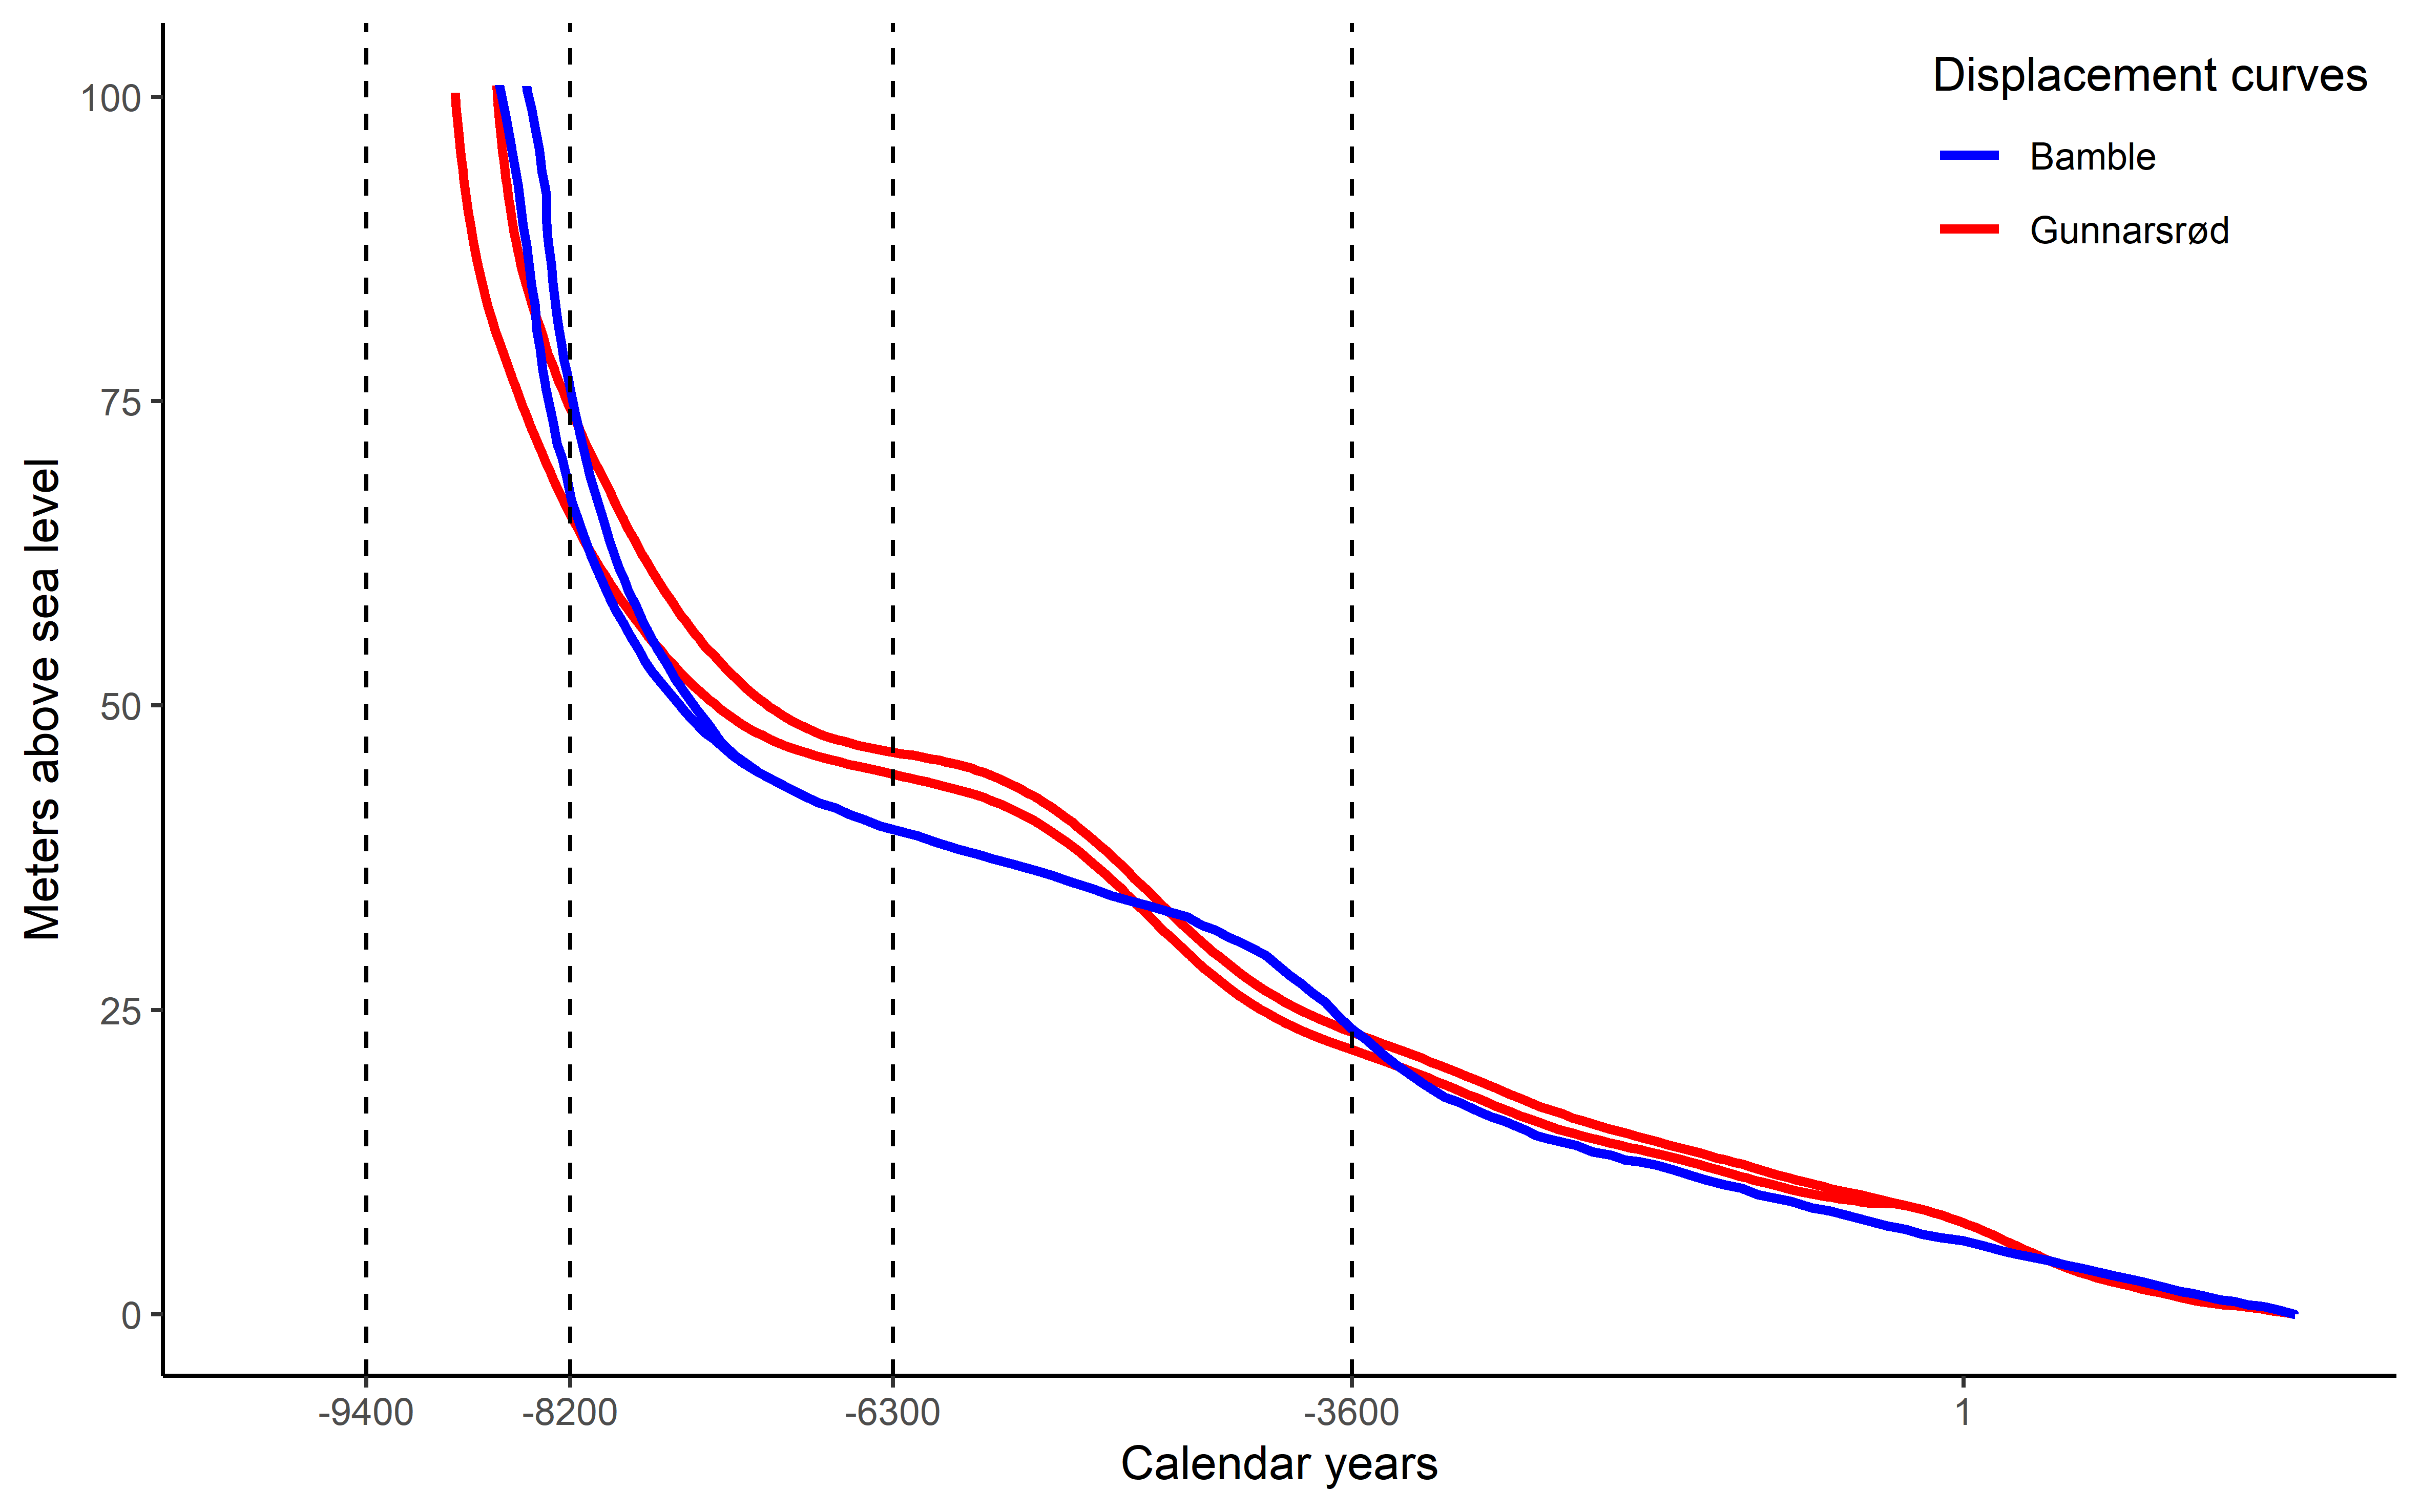
\includegraphics[width = \linewidth]{displacement.png}
	\caption{Shoreline displacement curves for the study region \citep[after][]{sorensen2014, sorensen2015}. The transitions between the chronological phases are given by the vertical lines. The Bamble curve covers Bamble municipality, and the Gunnarsr{\o}d curve Porsgrunn and Larvik (Figure \ref{fig:displacement}).}
	\label{fig:displacement}
\end{figure}

\section{Sampling scheme}
To understand where sites are located in the landscape ultimately also depends on our knowledge of where they are verifiably $not$ located, as this allows us to get at the degree of selectivity exhibited by prehistoric inhabitants \citep[][2]{jochim1989}. As Stone Age sites are typically discovered by means of test-pitting in southern Norway, surveys do not provide a continuous field of known presence or absence of archaeological material, and no verified negative data is readily available from sources such as $Askeladden$. Random samples of control points representing assumed non-sites were therefore generated across the landscape \citep[e.g.][]{kvamme1988, fisher1997}. These were first constrained to avoid areas with higher slope values than any of the sites. This was done both because surveys are commonly directed by degree of slope \citep[e.g.][369]{nielsen2016}, and because this excludes extremely steep areas unsuitable for human occupation. Similarly, the samples were also constrained to fall within the elevation range of the sites, as areas outside of this would not have represented alternative coastal locations in the Mesolithic. Finally, samples were restricted to avoid present day lakes, because several of these are likely to have been present or part of the sea in the Mesolithic, and because they are typically only partially surveyed when water levels are low.\par     
As the most substantial survey projects have followed from the expansion of infrastructure, this has led to severe spatial structuring in the retrieval of archaeological material. Two sampling frames were employed in an attempt to work around this issue. The first involved constraining the random sample by a 500 m buffer around the sites, in addition to the environmental constraints. This is somewhat arbitrary, but follows from the survey strategy that has been employed for highway projects, where a 400 m tract along the proposed highway is surveyed, with additional extensions for areas such as planned intersections and lay-bys \citep[][7]{eskeland2017}. The second sampling frame involved creating a convex hull around these buffers, in addition to the environmental constraints. This larger hull constraint is likely to include more variability in the background populations for the variables considered, but it is less certain that any observed pattern is not simply an effect of including areas in the analysis where no archaeological investigation has taken place \citep[cf.][217]{kvamme2020}. While the smaller buffer sampling frame is not a safeguard against this effect, and the considerable reduction in sample space is likely to exclude variability that was relevant for locational choices, any locational pattern that can be observed using both sampling schemes would result in a far more convincing result in terms of whether actual locational preferences have been discerned. The sample sizes were set at 1000 for each of the two sampling strategies for each of the three phases, totalling at 6000 random samples.\par

\section{Locational variables}
Below follows a presentation of the considered environmental covariates. These are mainly derived from previous informal studies of Mesolithic settlement patterns in Norway. Of these, exposure are among the most central and has been emphasised in studies undertaken in most areas of the country \citep[][]{bjerck2008, berghansen2009, aastveit2014}. Exposure is also the locational variable that has been most explicitly linked to mobility, where a common sentiment is that higher mobility is reflected in higher degrees of site exposure. As societies in earlier periods are typically understood to have been more mobile, the general trend is to be an overall decrease in site exposure through the Mesolithic \citep[e.g.][]{lindblom1984, jaksland2001, bjerck2008, breivik2018}. \cite{svendsen2014} has, however, pointed out that the exposure term as used in Norwegian Mesolithic research has referred to both lack of shelter from wind and sea, but also degree of visibility from sites. In an attempt to get at this distinction, exposure is treated by two variables. \par

\subsection{Wind fetch} 
Wind fetch is a fundamental concept in the study of ocean systems and environments that is commonly employed outside archaeology to estimate the exposure of locations to wind-generated wave action (\citealp[][]{laing1998}, \citealp[for archaeological applications see][]{nitter2013, nitter2018}). Wind-generated wave action is a complex phenomenon that can depend on a wide range of parameters. However, the most commonly applied models for wave exposure are founded in so-called fetch-based indices. Fetch is defined as the unobstructed distance of sea across which the wind travels towards a given location. The longer the uninterrupted distance the wind can travel the surface of the ocean, the higher waves will tend to be. Wave prediction models based on fetch involve various degrees of complexity, starting from relatively simplistic models that only take account of the length of the fetch, as is done here. While more complex models allow for more accurate predictions that also move beyond estimation of mere relative exposure \citep{malhotra2007, bekkby2008, sundblad2014}, investigations into the predictive power of fetch-based models have found that those based solely on fetch length still perform reasonably well in predicting the presence and absence of biological indicators of wave exposure \citep{burrows2008, hill2010}. \par
Here, estimation of average fetch length was based on the procedures presented by \cite{ekebom2003} and \cite{tolvanen2005}. With the sea-level raised just above each random point and the centre point for the site polygons, this involved first drawing a line every 7.5 degrees in circumference around each point. The lines were clipped by the raised coastline, and by the present day coastline in the larger region (Figure \ref{fig:fetch}). The average length of the lines were then returned. The coastline has also changed considerably outside of the study region throughout the Mesolithic, which means that the the average fetch of the more exposed locations has likely been underestimated. However, as the average fetch lengths will largely be determined by the immediate surroundings, this seemed like less of a problem for the purposes of mapping general locational patterns. \par

\begin{figure}[!htb]
	\makebox[\textwidth]{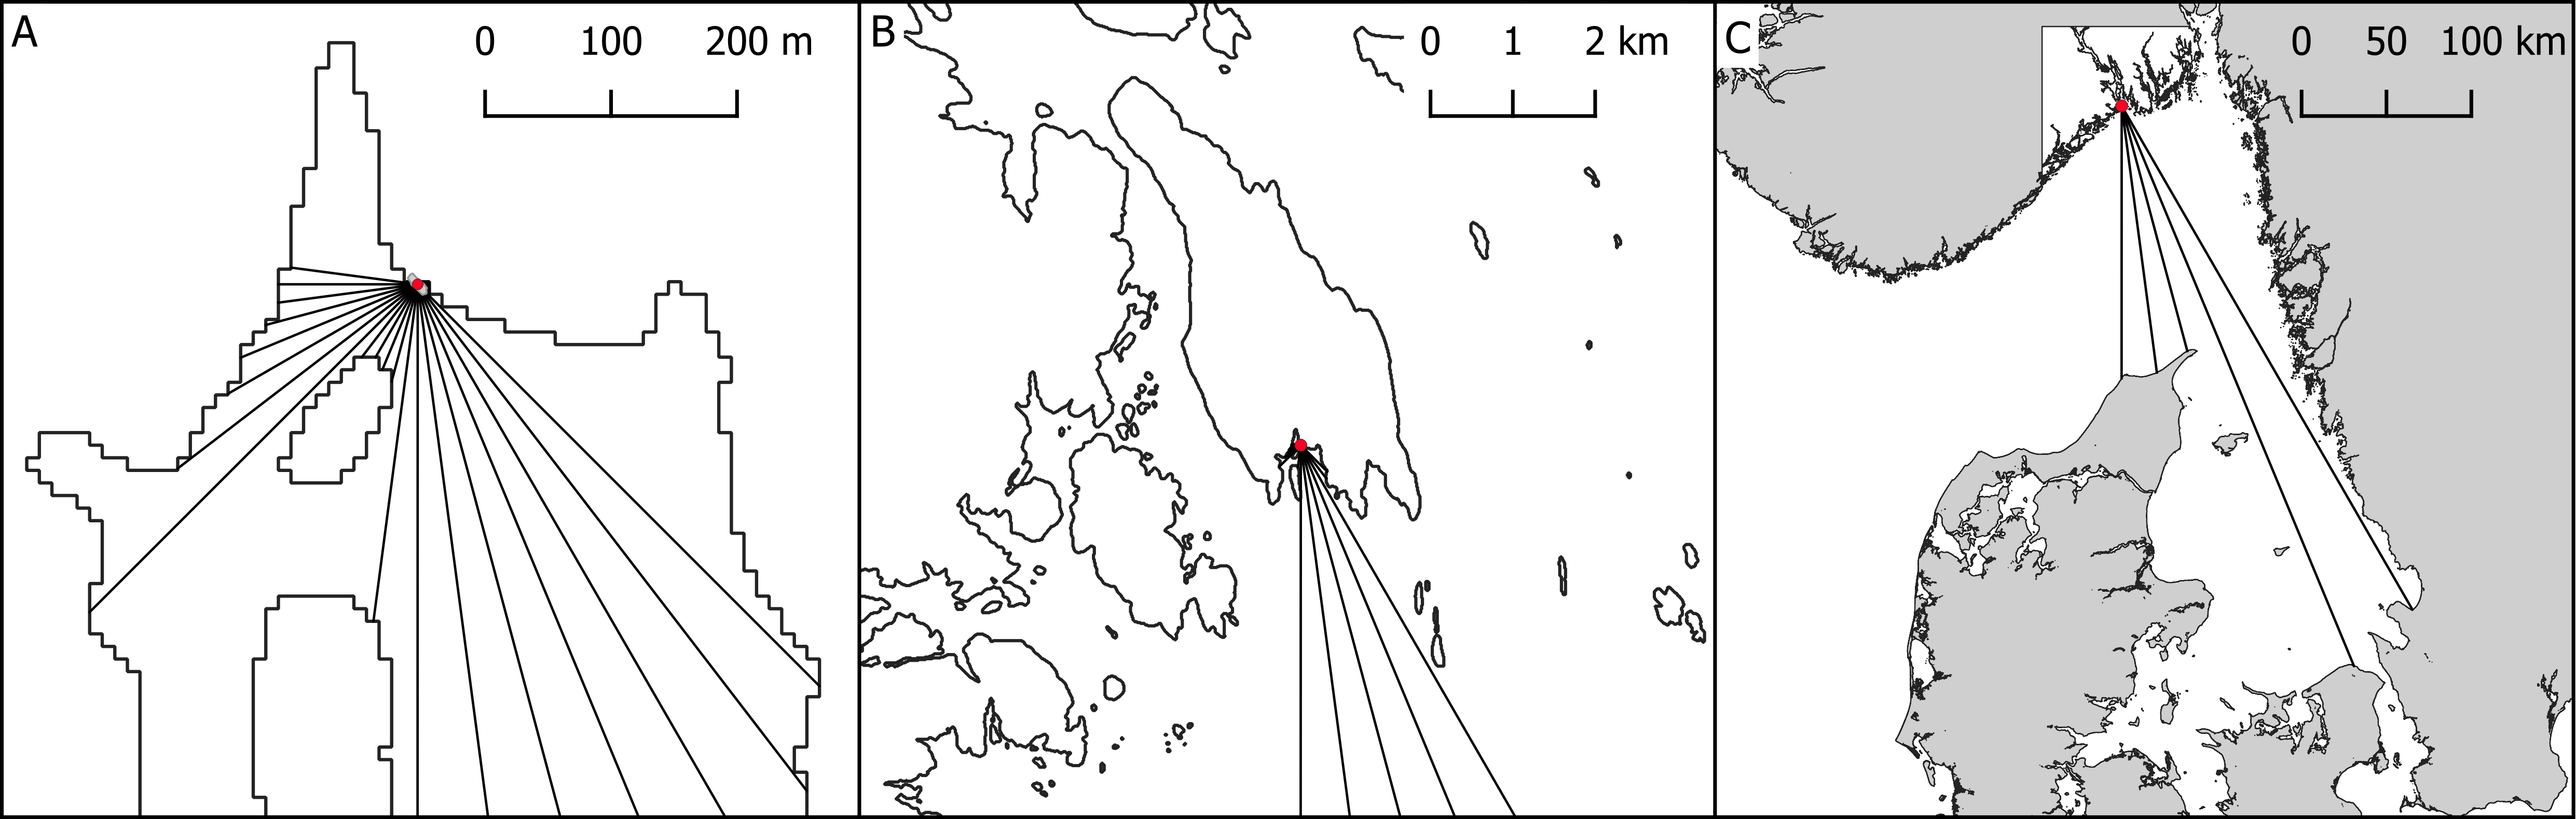
\includegraphics[width=1.3\textwidth]{fetch.png}}%
	\caption{Average fetch as estimated from site with Askeladden ID 22346-1. A) Sea-level has been raised to 34 meters above present. The lines are drawn from the point that is the average coordinate of the underlying site polygon. These are then clipped as they intersect the polygons representing land from the vectorised DTM with 10 m resolution. B) The five fetch lines that escape the inlet in which the site is located continue. C) Outside of the area covered by the regional DTM the present day shoreline is used for clipping the lines. This is based on a 25 m resolution DTM.}\label{fig:fetch}
\end{figure}

\subsection{Visibility}
Viewshed analysis was employed to investigate visibility patterns (\citealp[][225--233]{conolly2006}; \citealp{gillings2020}). As my interest here are general visibility patterns, simple measures of total visible area from the analysed locations was deemed sufficient. The outer radii of the viewsheds was set to 5000 and 10,000 meters to represent views at a long and medium distance. These distances are somewhat arbitrary, but relatively common when mapping the size of views where a target has not been defined \citep[e.g.][]{lake2000, lopez2008, garcia2013}. The elevation of the observer point was set to 1.65 m above ground, and r.viewshed, the employed GRASS module, was set to take the curvature of the earth into account. \par
The sea level was raised to the lowest elevation of each site polygon, and the viewsheds computed from the centre points. For raising the sea level to the random point locations, a circular buffer with a radius of 11.9 meters was generated around each point. This equates to the median site size. Results were returned as the number of cells visible from each point. \par

\subsection{Shoreline displacement}
\cite{wren2018} recently investigated the relationship between Wemindji settlement location and rapid isostatic rebound in James Bay, Canada. They found that the sites tend to be situated at locations where the topography will have resulted in a higher than expected degree of coastal stability within 2 km radius of the sites, and a higher than expected variability in shoreline emergence within 20 km of the sites. This is taken to reflect a settlement strategy favouring site locations with stable local surroundings that simultaneously offer ecological variability within wider resource catchments. Variation in when areas emerged from the sea means that these will be at various stages of ecological succession, following the transition from oceanic, to littoral, to terrestrial environments. \par 
A similar approach is taken here, with a few adjustments to the methodology. First, the shoreline displacement curves for the study region are only reasonably reliable up to around 100 masl. The 32 EM sites situated above 100 masl were consequently excluded from this part of the analysis. Furthermore, the shoreline displacement in south-eastern Norway cannot be approximated by a low-order polynomial. The maximum radius explored around sites and non-sites was therefore set to 1 km, simply due to uncertainty towards the outer edges of the distribution of sites. \par The emergence raster in Figure \ref{fig:emerge} was created by reclassifying the elevation raster based on the regional displacement curves. As the assumption here is that all sites have been situated on the shoreline, all areas lower than the lowest elevation of the site polygons and non-site buffers were excluded from analysis for each location. Standard deviation in year of emergence was then retrieved using buffers with radii of 50, 500 and 1000 meters around the point locations. \par

\begin{figure}
	\centering
	\includegraphics[width = \linewidth]{emergence.png}
	\caption{Reclassified elevation raster by year of emergence given in calendar years. The area west of the red line has been reclassified using the mean of the Bamble displacement curve, and the area to the east using the mean of the Gunnarsr{\o}d displacement curve (Figure \ref{fig:displacement}).}
	\label{fig:emerge}
\end{figure} 

\subsection{Island location}
Several authors have pointed to the fact that a substantial amount of sites seem to have been situated on small islands, and especially so in the earlier parts of the Mesolithic \citep[e.g.][]{nyland2012, bjerck2013, bjerck2017}. Behavioural explanations of this assertion has followed a general emphasis on boating and resource exploitation in archipelago environments, but has also been explicitly related to extensive seal hunting in the earliest part of the Mesolithic \citep{bjerck2017}, as well as concentrations of marine productivity in the lee of smaller islands \citep{breivik2014,schmitt2015}. For this analysis a context dependent algorithm available in the provided Python script was devised to identify if point locations would have been situated on islands, assuming they were shore-bound. If yes, then the size of the island was found.

\subsection{Sediments and infiltration ability}
Sites have also been suggested to be located relative to different soils and sediments \citep[][]{bergsvik1995, berghansen2009}. This suggestion is based on the assumed desire to situate sites on well-drained locations. The sediment data used here was retrieved from the Geological Survey of Norway and has a resolution of 1:50,0000. The sediment data has an infiltration score, relating to how well the sediments drain and clean wastewater. While these are in part related to the potential for biological breakdown of toxins, they are also determined by degree of permeability \citep{ngu2015}. Thus, while the original motivation for the classification does not perfectly align with my intended use, it does appear to capture the relevant properties of the sediments. The infiltration level for each site was found by taking the mode on each site polygon and each of the non-site buffers. 

\subsection{Aspect}
Aspect has also been suggested to be important to locational choices in Mesolithic Norway. This is typically seen in relation to shelter \citep[][47]{berghansen2009}, a desire to face either land or the open sea \citep{darmark2018}, or to situate sites at locations that receive more sunlight throughout the day (\citealp[][58]{mikkelsen1989}; \citealp[][113]{berghansen2009}). Here it was decided to focus on the possible relevance of aspect as related to sunlight, as the other proposed reasons for why aspect should be relevant should mostly be captured by other variables. The aspect of each location, returned as degrees from north, was therefore transformed to deviance from south by finding the absolute distance of each value from 180 degrees \citep[][]{spencer2018}. 

\section{Quantitative framework}
\subsection{Model building strategies}
The first statistical method applied is logistic regression, which forms the backbone of site locational analysis in archaeology. The most common approach to model building with regression methods in archaeology could be said to fall in the category of stepwise minimisation, sometimes also called data-driven model tuning, as this often starts with analysis of the relationship between predictors and the response, independently of the multivariate model \citep[][182--183]{conolly2006}. This becomes very problematic when variables are included or excluded from further analysis based on the statistical significance of this relationship, as has sometimes been the case (\citealp[e.g.][152--153]{stancic2000}; \citealp[][36]{duncan2000}). This is in effect a form of $p$-value driven, forward stepwise variable selection, and is hampered by severe issues \citep[][71--72]{harrell2015}. First of all this approach would exclude a variable without considering whether it might be an important predictor once other variables are controlled for, or if it might alter the effect of other predictors in the model. If such effects are present, the variable should be included in the model irrespective of whether or not it is a good predictor of the independent variable (\citealp[][416]{kohler1986}; \citealp[][89]{james2013}. Secondly, this method has a tendency to inflate model performance. This follows from the fact that the final model specification is typically evaluated using standard methods that do not take the model tuning process into account. Not accounting for the total number of variables considered, including those that were discarded, breaks the assumptions underlying most standard statistical hypothesis testing and estimation methods, leading to a deflation of $p$-values and confidence intervals, and an inflation of $R^2$ values and coefficients \citep{harrell2015}. \par
However, the term stepwise selection is typically taken to refer to a form of automated model selection that has also seen application in archaeology \citep[e.g.][]{bevan2013, visentin2017, spencer2018, wachtel2018}. Here, independent variables are excluded or included in the model at sequential steps that are stopped once a statistic that determines the relative success of the models does not improve. The Akaike and Bayesian information criteria (AIC and BIC, respectively) are the most frequently applied statistics for stepwise model selection in archaeology. Stepwise selection based on AIC and BIC are seen as an improvement over simple minimisation by use of $p$-values as a stopping criteria, as they take the total number of variables considered into account in the evaluation of the final model. The fundamental strategy of automated stepwise model selection has, however, received considerable criticism \citep[e.g.][]{henderson1989, derksen1992, chatfield1995, malek2007, burnham2011, harrell2015}, and the implications of multiple testing and model tuning are more profound and difficult to take account of in a satisfactory way, leading \citeauthor{harrell2015} (\citeyear[][69]{harrell2015}) to conclude that `AIC is just a restatement of the $p$-value, and as such, doesn't solve the severe problems with stepwise variable selection other than forcing us to use slightly more sensible $\alpha$ values.' \par
The most basic model building strategy associated with regression techniques is the forced entry, direct or simultaneous technique, where all independent variables are included from the start, with no consideration of the relative importance, or the order by which the variables should be included \citep[e.g.][]{stoltzfus2011}. This is typically best suited when there is little reason to hold any a priori assumptions about the nature of these aspects, and is the approach taken here. The main drawback of this approach is the danger of overfitting and including irrelevant variables that only contribute an increase in standard errors. \par
Given the dramatic increases in computational power over the last decades, iteratively fitting hundreds or even thousands of models has now become tractable. Faced with this, automated model specification through stepwise selection could appear to be one way to handle this flood of information. Furthermore, regression models can offer insight into the complex net of relative and absolute variable importance, the relationship between these, and an estimate of the confidence with which these assertions can be made. But, as shown above, several authors have argued that this potential is lost with the implementation of stepwise model selection. To fully utilise their capacity arguably requires decisive and rigorous implementation of a well-thought-out, thorough and at times time-consuming modelling strategy \citep[e.g.][94--99]{harrell2015}. It could perhaps be argued that in the face of a fragmented and sparse material such as that frequently encountered in archaeology, a looser and more exploratory modelling procedure is warranted. \cite{woodman2002} have argued the precise opposite. They contend that this uncertainty is precisely where careful modelling is most necessary and beneficial, as this can help both elucidate the nature of the fragmentation and guide an analysis that could otherwise be led astray.\par
Relevant to this is the delineation that \cite{breiman2001a} makes between what he terms a data modelling culture and an algorithmic modelling culture in statistics. The data modelling culture is based on an assumption that the data under study represents independent draws from a data-generating process where the value on a response variable follows a stochastic model of the form $f$(parameters, predictor variables, random noise). The algorithmic modelling culture, on the other hand, only makes the assumption that the data represents independent results of a complex and mostly unknowable underlying multivariate process. The goal is to identify an algorithm that best predicts the outcome of this underlying process. Good prediction indicates a better emulation of the underlying process than a solution that predicts poorly. A normal criticism of this focus is that prediction is not explanation, and that despite predictive success, the algorithms in use are often too impenetrable to contribute much in the way of explanation. \citeauthor{breiman2001a} (\citeyear[][210]{breiman2001a}) states that this dichotomy of interpretability and explanation as opposed to prediction is contrived: `The goal is not interpretability, but accurate information'. While regression models can offer a highly interpretable output in the form of coefficients and confidence intervals, they are argued to be easily distorted by resting on assumptions concerning the nature of the underlying distributions that are virtually never met in the analysis of real world phenomena. Additionally, they appear to often be outperformed when it comes to prediction. While the output of machine learning techniques is less interpretable, it is certainly less opaque than the original process under study. Hence, it is argued, they can provide far more reliable and accurate insight, even if this insight holds less detail. \par

\subsection{Random forests}
Relatively high predictive power, ease of implementation and its non-parametric nature are among the elements that have led to the popularity of random forests \citep[][587--604]{hastie2009}. Random forest is an ensemble method that leverages the increased predictive power following from aggregating the results of a large number of de-correlated, high-variance, low-bias decision trees \citep{breiman2001b}. Decision trees for classification are based on identifying what variables best partition the data into classificatory groups at sequential binary splits \citep[][116--118]{baxter2003}. At each split the variable to use is decided based on how well the candidate variables partitions the data into the correct groups. The degree of discriminatory success is also termed purity, and is often given by the Gini impurity score, which represents how often a random observation would be labelled incorrectly on the given split. While classification trees are highly interpretable and often perform well in classifying the original training data, they have a tendency towards high variance \citep[][312]{hastie2009}. \par
To avoid overfitting while reducing the amount of variance, random forest works by combining bootstrap aggregation of the training data with a random selection of predictor variables to be used in the construction of each individual tree (Box \ref{rf}). Thus, for each tree the training data is first randomly redrawn with replacement, which results in around $2/3$ of the original data being evaluated in the training of the entire forest---a process also known as bagging. The remaining $1/3$ is known as the out-of-bag (OOB) sample, and can be used for subsequent model validation and variable importance estimates. Following each resampling, a classification tree is grown. For each node in the tree, a random subset of predictors is drawn, and the predictor returning the lowest Gini impurity score is selected at that node split. The number of randomly selected predictors evaluated at each node is recommended to start at $\sqrt{p}$ for classification trees, where $p$ is the number of independent variables. The number of variables to be evaluated at each split, the parameter $mtry$, is then explored during model tuning. As there is no danger of overfitting associated with generating too many trees, the arbitrarily large number of 5000 trees were generated for each forest here. While this came at a computational cost, it meant only the $mtry$ parameter required tuning. \\

\noindent\fbox{%
	\parbox{\textwidth}{%
		\captionof{boxing}{Random Forest for classification \citep[modified from][588]{hastie2009}.\label{rf}}
		1. For $B$ bootstrap samples $b = 1,...,B$:\par
		\-\hspace{1cm}a) Draw sample Z* of size $N$ from training data $X$ with replacement.\par
		\-\hspace{1cm}b) Grow tree $T_{b}$ by iterating over nodes:\par
		\-\hspace{2cm}i. Select $m$ random variables from $p$ predictors.\par
		\-\hspace{2cm}ii. Select variable giving the best split.\par
		\-\hspace{2cm}iii. $if$ split reduces impurity:\par
		\-\hspace{3cm}Split the node into two new nodes.\par
		\-\hspace{2cm}iiii. $else$:\par
		\-\hspace{3cm}Define as terminal node.\par
		2. Output classification tree ensemble $\{T_{b}\}^{B}_{1}$.\medskip
		
		Random forest prediction at point $x$ is then given as \^{C}$^{B}_{rf}(x) = majority\ vote$
		\{\^{C}$_{b}(x)\}^{B}_{1}$, where \^{C}$_{b}(x)$ is the prediction of the $b$th classification tree.\\ 
		
	}%
}\\ 

An important output of random forests is the variable-importance estimates that rank the variables based on their ability to correctly classify the input data. Following \cite{parr2018}, variable importance was here found by means of the permutation importance method. This is based on first running the OOB-sample through the final forest to establish the baseline accuracy. Then the column of values for a independent variable is randomly shuffled, and the OOB-sample is run through again. The difference in accuracy between the two runs then gives the variable importance measure. It is crucial to note that these can only be used to evaluate the relative importance of variables, and do not provide estimates of effect size. \par

\subsection{Model validation}
Internal model validation was done by means of bootstrap resampling for the logistic regression models \citep[][]{kvamme1988, verhagen2009}. The purpose of applying this method is to replace distributional assumptions and asymptotic results with computationally derived confidence intervals \citep[][605]{fox2008}, and to avoid both fitting and evaluating model performance using the exact same data \citep[][249--254]{hastie2009}. This entailed iteratively resampling the original data and fitting each model 9999 times. For each iteration the coefficients were retrieved, in addition to the Brier score and Area under the receiver operating curve (AUC). The Brier score is what's knowns as a proper accuracy score as it summarises calibration, the difference between the predicted probability and the observed probability of an outcome, as well as model resolution, the spread of the predictive distribution \citep{rufibach2010}. The measure ranges from 0 to 1, where 0 represents perfect accuracy. The score is not especially meaningful on its own, however, and is best suited for comparative purposes. The AUC score has a more intuitive interpretation than the Brier score, but only considers the discriminatory abilities of the model \citep[173--182]{hosmer2013}. The AUC ranges from 0 to 1, where 1 represents perfect classification, and 0.5 represents no improvement over random classification. The accuracy scores are reported as the mean result across bootstrap samples. The coefficients were evaluated by means of 95\% bootstrap percentile intervals, constituted by the range between the $2.5th$ and $97.5th$ percentiles of coefficient values generated across the bootstrap samples \citep[][595]{fox2008}.\par
Variable importance estimates and model performance measures for the random forests were found using nested $k$-fold cross-validation instead of the bootstrap (Box \ref{cv}, and below for imputation of missing values). The reason for this is that while the logistic regression models were fit using the simultaneous technique, a model tuning step was included for the random forests to identify the optimal number of random variables to be evaluated at each split in the classification trees (the parameter $mtry$). Single bootstrap resampling results in some overlap between the original data and the resampled observations, meaning tuning and validating with this technique would likely lead to overfitting and overestimation of model performance \citep[][250]{hastie2009}. Basic cross-validation involves randomly splitting the data into $k$ folds, training the model using all but one fold, and then validating the result against the retained fold (\citealp[92]{verhagen2009}; \citealp[][241--249]{hastie2009}). This is then repeated until each fold has been used as the validation set. The nested version of cross-validation entails that for each of these validation steps the folds not retained are split into an additional $k$ folds. Here a complete sweep of possible $mtry$ settings was done for each inner cycle, and the $mtry$ achieving the best performance by means of AUC was returned and used for the current outer fold. The final AUC and Brier scores, as well as variable importance measures are reported as averaged across the outer validation cycle.\\

\noindent\fbox{%
	\parbox{\textwidth}{%
		\captionof{boxing}{Nested 5-fold cross-validation of random forests.\label{cv}}
		For each of 5 imputed datasets:\par
		\-\hspace{1cm}1. Randomly split into 5 outer folds. \par
		\-\hspace{1cm}2. For each outer fold:\par
		\-\hspace{2cm}a. Split the other 4 outer folds into 5 inner folds.\par
		\-\hspace{2cm}b. For each inner fold:\par
		\-\hspace{4cm}i. For $P$ predictors $mtry = 1,...,P$: \par
		\-\hspace{5cm} Create random forest using $mtry$.\par
		\-\hspace{4cm}ii. Return $mtry$ achieving highest AUC score.\par
		\-\hspace{2cm}c. Return $mtry$ achieving the highest AUC across inner folds. \par
		\-\hspace{2cm}d. Run random forest using optimal $mtry$ on outer fold.\par
		\-\hspace{2cm}e. Report Brier score, AUC score and variable importance. \par
		\-\hspace{1cm}3. Return mean Brier, AUC and variable importance from outer folds.\par
		Return mean Brier, AUC and variable importance from imputed datasets.
	}%
}\\

\subsection{Model parameters and preprocessing}
Below follows a presentation of predefined model parameters and the preprocessing steps that were taken. With the exception of for imputation, the response variable was kept out of this process to maintain inferential validity.\par
Apart from aspect deviating from south, all continuous variables were transformed for the logistic regression models by taking the natural logarithm due to extreme distributions. Continuous variables were then normalised to take on values between 0 and 1 to better facilitate a comparison of the impact of each variable, although at the cost of distorting the interpretability of effect sizes \citep[cf.][]{spencer2018}. In the random forests, the variables were included using raw values. For a second set of models directly comparing the location of sites between the different phases, as opposed to sites and non-sites, all variables with the exception of the binary island/mainland variable were transformed by finding the percentile rank of each site value as compared to the values in the corresponding hull sample. In an attempt to achieve more sensible diachronic comparisons, this adjusted the values by variation in the surrounding landscape as captured by the hull samples for each phase.\par
There are a host of different methods for identifying and dealing with collinearity \citep[e.g.][]{dormann2012, tomaschek2018}. The approach taken here was a relatively straightforward one, where Pearson's $r$ and Spearman's $\rho$ was found for each predictor variable pair for each chronological phase. In the case of problematic levels of correlation between predictor variables across all phases ($|r\ or\ \rho| > 0.8$), all but one of the correlating variables were removed from analysis. The choice of what variable to retain was based on what variable appeared to best summarise the collinear group in substantive terms (Table \ref{table:var}).\par
Following the lack of previous quantitative studies on which to base this analysis, linearity with the logit could not reasonably be assumed for the predictors in the logistic regression models. To allow for non-linearity, pre-specified natural splines with default quantile knots could have been included \cite[][26--28]{harrell2015}. However, with 104 sites for the EM representing the smallest effective sample size, the inclusion of more than 10 model parameters would likely lead to overfitting, following the most lenient $m/10$ rule provided by \citet[][72--73]{harrell2015}, where $m$ is effective sample size. Consequently, as there were no grounds on which to prioritise among variables to include with splines, none were used. Similarly, due to the large number of possible two-way interaction effects, no interaction terms were included in the models as there were no grounds on which to prioritise among these \citep[cf.][36--38]{harrell2015}.\par 
In total, shoreline emergence was missing for 32 sites and 725 non-sites, while infiltration level was given as unclassified for one site and 138 non-sites. Imputation of these missing values was deemed most appropriate. Unless the number of cases that have missing data is very low, or the values are missing completely at random, which is rarely the case, the alternative of deleting observations can lead to dramatic loss of information and bias in all model estimates \citep[][]{nakagawa2008}. Imputation for the logistic regression models was done using predictive mean matching \citep{buuren2011}. This is based on performing OLS-regression on the column with missing values, using the other variables in the data as predictors. From the resulting coefficients a random draw is then made, and these coefficients are used to predict the entire column containing missing values, including those values that are not missing. Each missing value is then given the originally observed value of one of its predicted closest neighbours by a random draw, typically among the five closest cases. This process is then ideally repeated multiple times, and subsequent analysis is based on a pooling of the results from running each imputed dataset through the full analysis. As the imputations done for the logistic regression were to be nested in a bootstrap, a single imputation was performed per bootstrap sample \citep{brand2018}. \par
Random forest provides its own method for imputing missing values based on its proximity and classification capabilities \citep{breiman2003}. This works by first setting the missing values to the average of the column and then growing and running the dataset through a random forest. For each classification tree in the forest, each observation that ends up in the same terminal node as the observation with the missing value is counted as similar. The value to be imputed is then given as the average across the proximal observations, weighted by the number of times they ended up in the same terminal node. This entire process is then repeated using the new values instead of the column average. Here five sequential random forests were grown, with each forest growing 5000 trees. This process was then repeated five times, creating five imputed datasets that each were run through the estimation and validation process described above.\par 

\begin{table}
	\hskip-2.0cm\begin{tabular}{ | l | l | l | l | l |}
		\hline
		Variable & Abbreviation & Measure & Collinearity & New name \\ \hline
		Location (island/mainland) & loc & 0 = island, 1 = mainland &&  \\ \hline
		Island size & isl\_si & Continous && \\ \hline
		Infiltration ability & infil & Ordinal 1--4 &&\\ \hline
		Deviation from south & dev\_south & Continous &&\\ \hline
		Average fetch & fetch &  Continous &&\\ \hline
		Viewshed 5 km &  view\_5  & Continous & A: + & view \\ \hline
		Viewshed 10 km &  view\_10  & Continous & A: - &\\ \hline
		Emergence 50 m  & emerg\_50 & Continous & B: + & emerg\_shdist \\ \hline
		Emergence 500 m & emerg\_500 & Continous & B: - &  \\ \hline
		Emergence 1 km & emerg\_1k & Continous & B: + & emerg\_lgdist \\ \hline
		\hline
	\end{tabular}
	\caption[Variable names and handling of collinear variables.]{Variable names and handling of collinear variables. Letter indicate collinearity group and + indicates that the variable was retained and used to represent the group in subsequent analysis.}
	\label{table:var}
\end{table}

\begin{figure}
	\makebox[\textwidth]{\includegraphics[width=1.5\textwidth]{em_hull_fig.png}}%
	\caption[Early Mesolithic - Hull sample]{Early Mesolithic - Hull sample. A) Map overview. B) Logistic regression, percentile bootstrap. C) Random forest, permutation variable importance.}
	\label{fig:em_hull}
\bigbreak
	\makebox[\textwidth]{\includegraphics[width=1.5\textwidth]{em_buff_fig.png}}%
	\caption[Early Mesolithic - Buffer sample]{Early Mesolithic - Buffer sample. A) Map overview. B) Logistic regression, percentile bootstrap. C) Random forest, permutation variable importance.}
	\label{fig:em_buff}
\end{figure}

\begin{figure}
	\makebox[\textwidth]{\includegraphics[width=1.5\textwidth]{mm_hull_fig.png}}%
	\caption[Middle Mesolithic - Hull sample]{Middle Mesolithic - Hull sample. A) Map overview. B) Logistic regression, percentile bootstrap. C) Random forest, permutation variable importance.}
	\label{fig:mm_hull}
\bigbreak
	\makebox[\textwidth]{\includegraphics[width=1.5\textwidth]{mm_buff_fig.png}}%
	\caption[Middle Mesolithic - Buffer sample]{Middle Mesolithic - Buffer sample. A) Map overview. B) Logistic regression, percentile bootstrap. C) Random forest, permutation variable importance.}
	\label{fig:mm_buff}
\end{figure}
	
\begin{figure}
	\makebox[\textwidth]{\includegraphics[width=1.5\textwidth]{lm_hull_fig.png}}%
	\caption[Late Mesolithic - Hull sample]{Late Mesolithic - Hull sample. A) Map overview. B) Logistic regression, percentile bootstrap. C) Random forest, permutation variable importance.}
	\label{fig:lm_hull}
\bigbreak
	\makebox[\textwidth]{\includegraphics[width=1.5\textwidth]{lm_buff_fig.png}}%
	\caption[Late Mesolithic - Buffer sample]{Late Mesolithic - Buffer sample. A) Map overview. B) Logistic regression, percentile bootstrap. C) Random forest, permutation variable importance.}
	\label{fig:lm_buff}
\end{figure}

\section{Results}
The results from comparing sites and non-sites are given in Figures \ref{fig:em_hull}--\ref{fig:lm_buff} and the results from comparing the different phases in Figures \ref{fig:em_lm}--\ref{fig:mm_lm}. It is striking that the two different sampling frames for non-sites largely return coinciding results for each phase, and that apart from some minor fluctuations, the random forests and logistic regression models perform about equally well. It is worth repeating that this has not been a controlled and balanced test of their potential performance, not least because the methods were subjected to different validation procedures. Confirming the findings by use of methods with different strength and weaknesses is nonetheless a benefit as this makes the final results more robust, and in the case of discrepancies, more nuanced. This is especially true as the sample sizes did not allow for much complexity in the logistic regression models.\par
Moving on to the substantive results, \citet[][177]{hosmer2013} state that AUC scores from 0.6--0.8 could generally be taken to indicate poor to acceptable discrimination, which is achieved when comparing sites to non-sites across all results given in Figures \ref{fig:em_hull}--\ref{fig:lm_buff}. This indicates that while the included variables are capturing some amount of patterning associated with the sites, a lot remains unexplained. The two exposure variables is driving most of the achieved result. This is irrespective of phase and whether the samples are from the hull or buffer constraints, and is evident in both variable importance estimates for the random forests and the coefficients of the logistic regression models. This is with the exception of the viewsize coefficient for the LM, which, while also tending towards positive values, is not significantly different from zero. The otherwise consistent nature of the relationship between view size and fetch length is somewhat surprising, however, where the coefficients indicate that larger view sizes and smaller average fetch lengths characterises the location of the sites. This pattern could consequently speak to a settlement strategy that favours open immediate surroundings that at the same time are sheltered from larger expanses of open sea. When sites are compared across phases using the percentile rank adjusted values, the exposure variables have a steady impact around zero, indicating that this is a fairly stable pattern throughout the Mesolithic.\par 
While the only consistently significant variables for the EM is related to the exposure of sites, both the MM and LM sites have a tendency to be situated in locations with a high degree of variation in shoreline emergence in close proximity around the sites. The LM sites additionally display a tendency to have stable surroundings within the larger of the considered catchments. The most immediate behavioural implication of this result could be that the sites in both phases represent locations from where resources within a short distance were exploited, as this points towards ecological variation in close proximity of the sites. One perspective might also follow from the fact that the shoreline emergence variables are based on a transformation from elevation to year of emergence, which means that they are not entirely divorced from the relief of the local landscape, or possibly, depending on if the sites were strictly shore-bound or not, bathymetry. An implication of this finding could consequently be that the variation in the immediate proximity of the MM and LM sites is related to good fishing grounds \citep[][]{darmark2018}. The relevance of the significantly stable wider catchments in the LM could then be that this reflects a more predictable pattern for the exploitation of flora and fauna. As it is not treated directly here, a possible increase in the relevance of bathymetric variation in the MM and LM has to be left as a suggestion, however, and the nature of the apparent relevance of shoreline emergence as a whole could clearly benefit from being evaluated while also considering bathymetric and topographic variation directly. \par

\begin{figure}[ht]
	\centering
	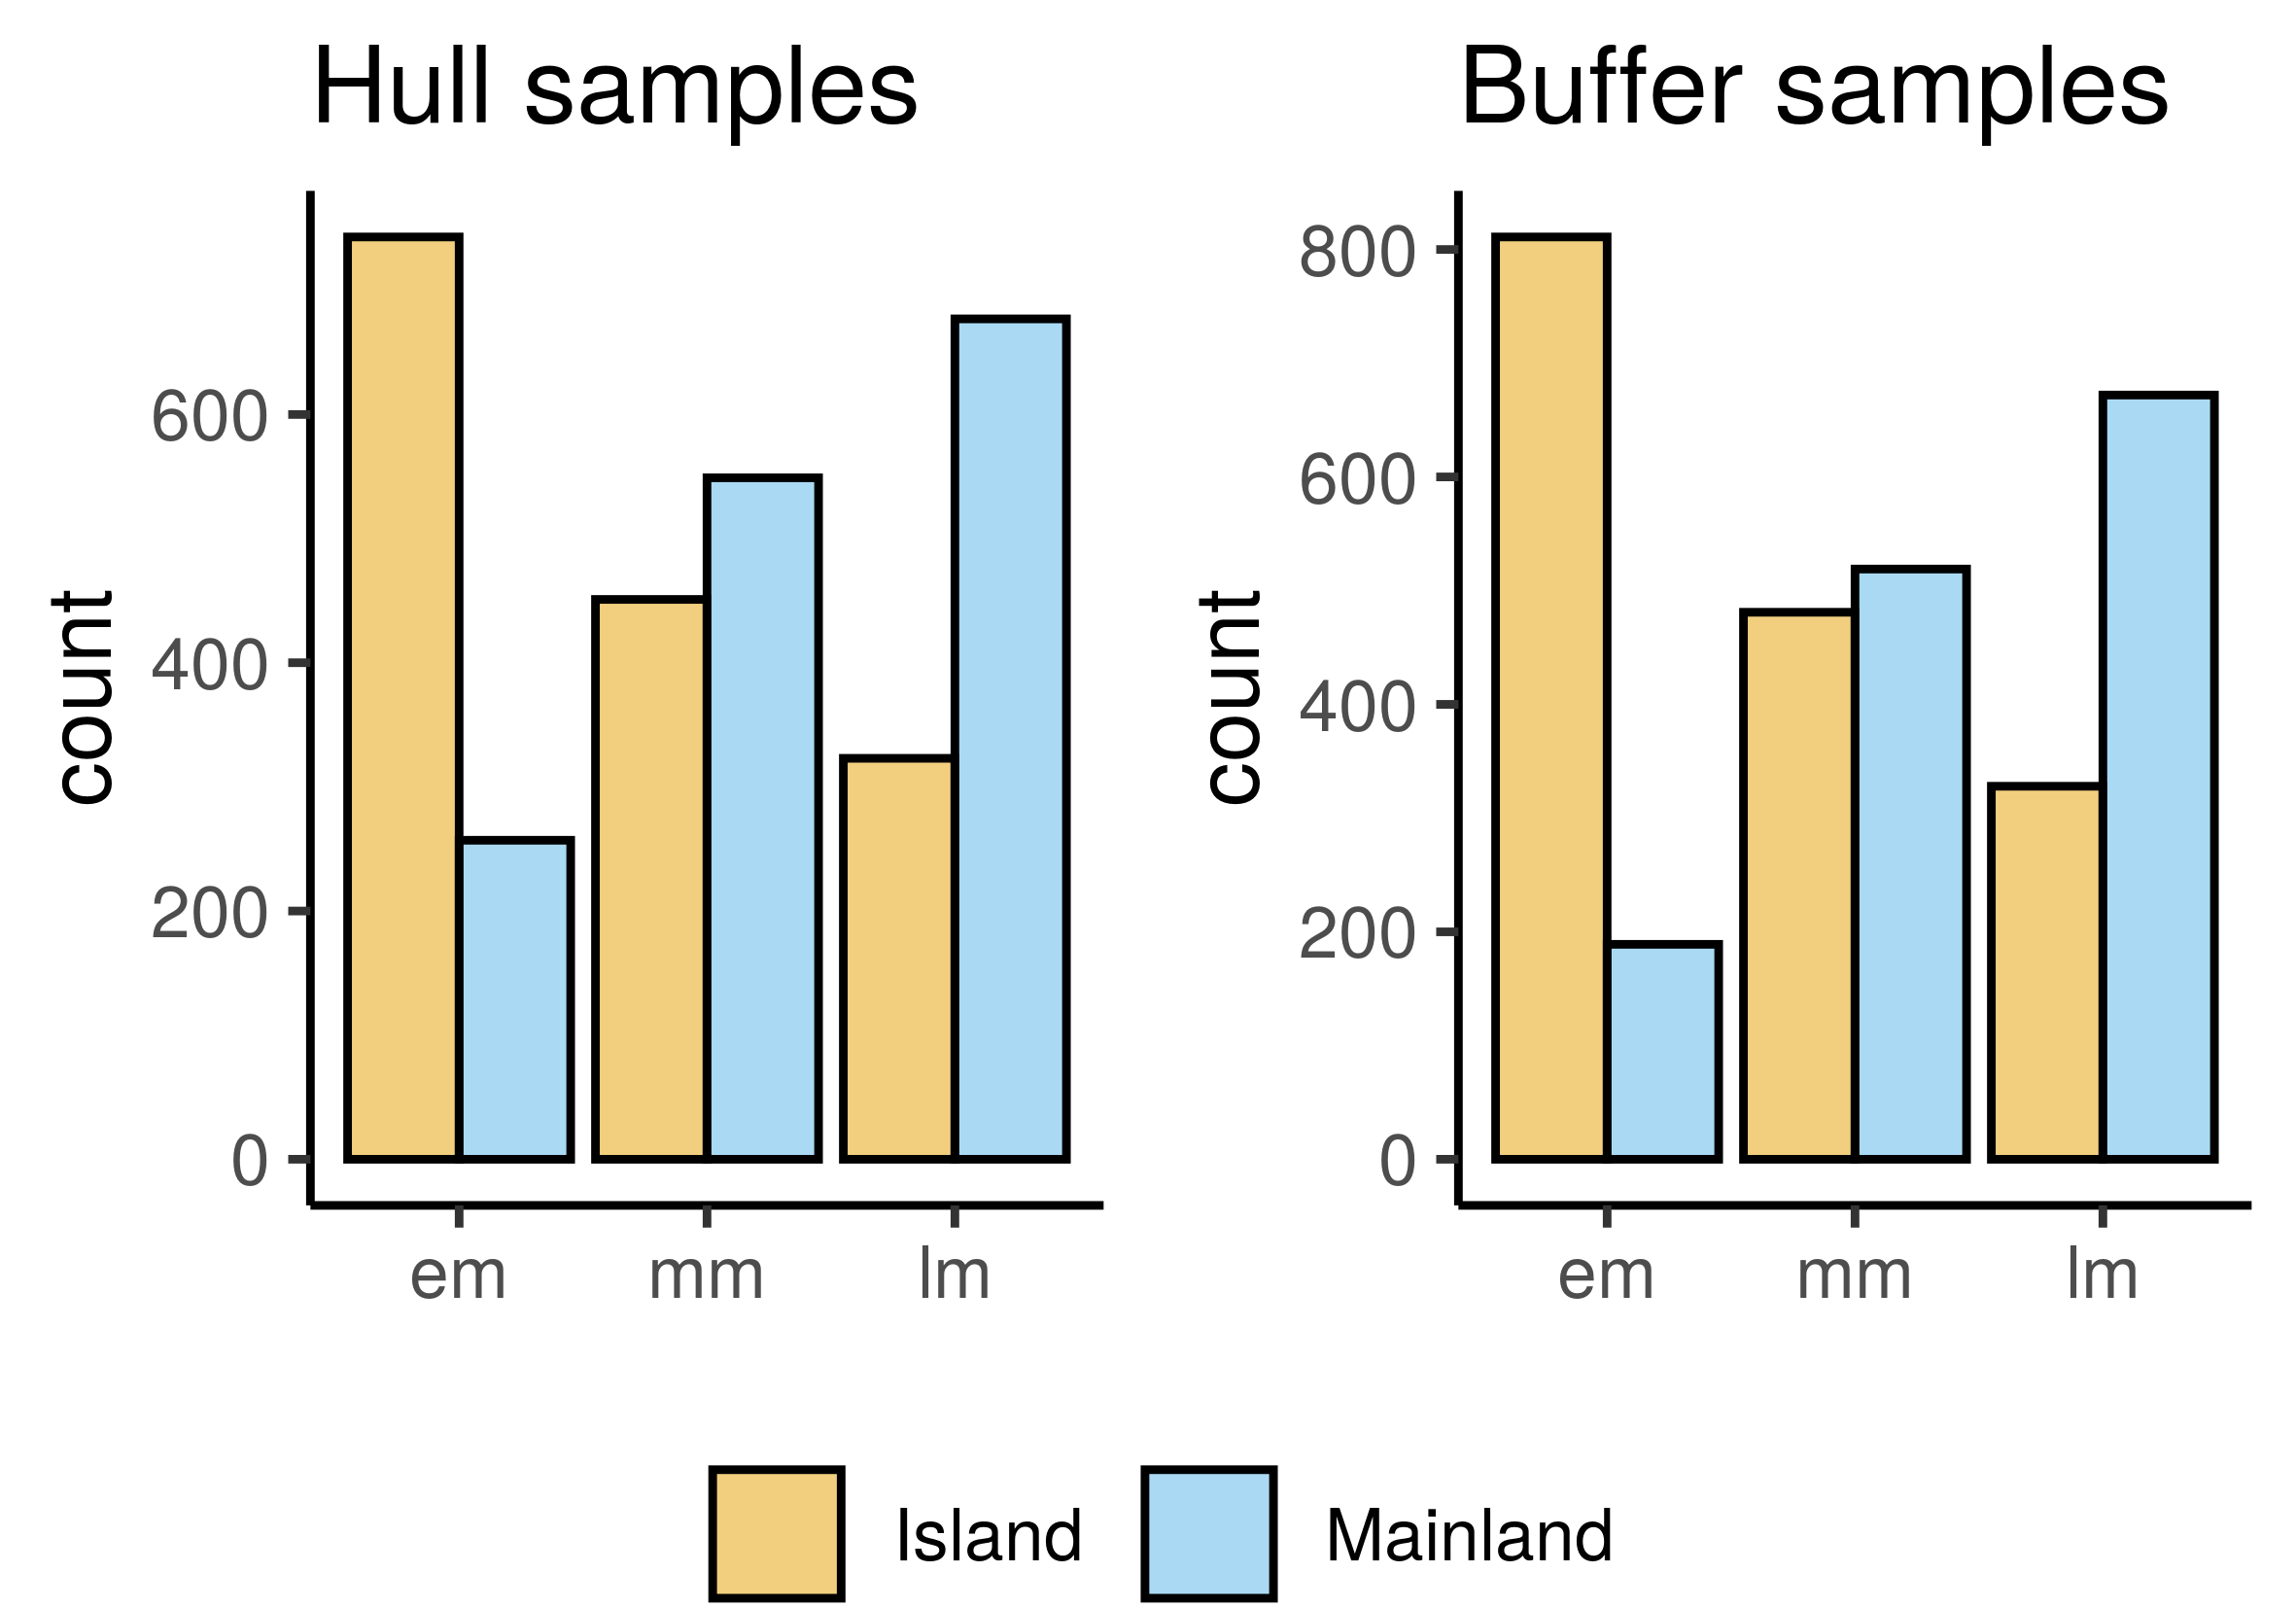
\includegraphics[width = 0.75\linewidth]{island_hist.png}
	\caption[Island/mainland among samples]{Number of random samples on islands and mainland across the different phases. It is evident that this proportion has varied dramatically throughout the Mesolithic.}
	\label{fig:island_hist}
\end{figure}

For the second set of models that compares the location of sites across phases, the island variables drove most of the result due to the fact that the number of islands has varied dramatically throughout the Mesolithic (Figure \ref{fig:island_hist}). The results were therefore plotted leaving out the island variables to make the comparisons between the other variables discernable in the plots while still taking account of their effect. In addition, the accuracy scores are given as the accuracy achieved by the two island variables subtracted from the accuracy achieved by the full model. The few significant coefficients in these models have minute effect sizes and the variables apart from the island variables only contribute minute changes in the accuracy scores. This indicates that the settlement patterns, excluding the island variables, largely coincide across all phases. Furthermore, following the logistic regression models comparing sites to non-sites, only sites from the MM appear to have a consistent significant propensity towards being situated relative to islands, where these have been slightly favoured, and sites have a higher tendency to be situated on smaller islands than could be expected by chance (Figure \ref{fig:mm_hull}--\ref{fig:mm_buff}). While the corresponding random forests do not place as much emphasis on these variables, this might be caused by some collinearity between the variables, causing their importance to be split between the two. Their impact is, however, relatively small even when combined, which could indicate that even though significant in the logistic regression models, the island variables might not have been of a huge importance in the MM.

\begin{figure}
	\makebox[\textwidth]{\includegraphics[width=1.5\textwidth]{em_mm_fig.png}}
	\caption[Early Mesolithic - Middle Mesolithic]{Early Mesolithic - Middle Mesolithic. The two island variables have been excluded from the plots, and the accuracy scores are given as the difference between that achieved by the full model and only by the island variables. A) Map overview. B) Logistic regression, percentile bootstrap. C) Random forest, permutation variable importance.}
	\label{fig:em_mm}
\bigbreak
	\makebox[\textwidth]{\includegraphics[width=1.5\textwidth]{em_lm_fig.png}}
	\caption[Early Mesolithic - Late Mesolithic]{Early Mesolithic - Late Mesolithic. The two island variables have been excluded from the plots, and the accuracy scores are given as the difference between that achieved by the full model and only by the island variables. A) Map overview. B) Logistic regression, percentile bootstrap. C) Random forest, permutation variable importance.}
	\label{fig:em_lm}
\end{figure}

\begin{figure}
	\makebox[\textwidth]{\includegraphics[width=1.5\textwidth]{mm_lm_fig.png}}
	\caption[Middle Mesolithic- Late Mesolithic]{Middle Mesolithic - Late Mesolithic. The two island variables have been excluded from the plots, and the accuracy scores are given as the difference between that achieved by the full model and only by the island variables. A) Map overview. B) Logistic regression, percentile bootstrap. C) Random forest, permutation variable importance.}
	\label{fig:mm_lm}
\end{figure}

A shift from a resource base focused on the hunting of sea mammals towards a wider subsistence spectrum including the regular exploitation of birds, undulates, shellfish and especially an intensification of fishing, is a gradual development believed to characterise the Norwegian Mesolithic \citep{breivik2014, bjerck2016, mjaerum2020}. Furthermore, a transition to a more diverse marine economy centred around fishing has been argued to have major implications for the mobility and settlement strategies of coastal hunter-gatherers, where such a shift could indicate a decrease in mobility \citep[e.g.][]{boethius2017, boethius2018}. The location of MM and LM sites with respect to variation in shoreline displacement, as identified in this study, could therefore be consistent with economic diversification and a decrease in mobility. However, the negligible performance measures and effect sizes in the comparison between phases given in Figures \ref{fig:em_lm}--\ref{fig:mm_lm} do not allow for the conclusion that any dimensions of the settlement patterns underwent consequential changes between the three considered phases. Furthermore, the importance of the shoreline displacement variables is limited compared to the other elements of the models comparing sites and non-sites, which instead suggest that shelter from the elements and open local surroundings has been more important, and fairly consistently so throughout the Mesolithic. This is with the exception of the logistic regression models for the LM, which, unlike the corresponding random forests, places more weight on the shoreline displacement variables. As noted above, the nature of this result requires further investigation. Nonetheless, the effect sizes for the two exposure variables are comparable across all phases, and in the comparison between phases the variables have a relatively steady impact around zero, indicating that site location relative to exposure has been similar in all phases. Thus, if degree of site exposure is taken to be a reflection of the economic basis for settlement, as has also been proposed \citep{bjeck2009, breivik2014}, the patterns discerned here would indicate a stable subsistence base throughout the Mesolithic. An alternative explanation to the apparent stability in settlement patterns could of course also be that these might simply not be sensitive to changes in the subsistence patterns of coastal hunter-fisher-gatherers in the archipelago environment of south-eastern Norway, and that this setting demanded that settlement patterns take on a distinct form, irrespective of variation along other social and cultural dimensions. One possible reason for this could perhaps follow from a dependency on boating that this setting is likely to have represented \citep[][]{glorstad2013}. This might, in turn, have contributed to a constraint on available variation space for locational strategies. It is, however, important to underscore that the limited performance of the models do mean that while no conclusion of clear diachronic difference can be drawn, this does not mean that the settlement patterns were necessarily the same---a considerable amount of variation does remain unaccounted for.

\section{Conclusion}
This study was aimed at elucidating general settlement patterns among coastal sites from the Mesolithic of south-eastern Norway through statistical modelling and algorithmic classification. The main substantive contribution pertains to the discerned importance of shelter from larger expanses of open sea while at the same time having open immediate surroudings, as well as the failure to identify any major diachronc differences in the locational patterns as a whole. While this final point is not a robust finding given some fluctuations in the shoreline displacement variables and the overall limited model performances, it is nonetheless an indication that the clear changes in settlement patterns that are to take place over time might have been exaggerated in earlier studies. This is given further support by the fact that site exposure has been emphasised as one of the major ways in which locational patterns are to have varied throughout the Norwegian Mesolithic \citep[e.g.][]{breivik2014}. This variation is not found for sites treated here. Taking a cue from \cite{aastveit2014}, this should suggests that instead of implicitly seeing these societies as situated somewhere on a linear trend-line moving towards ever increasing degrees of sedentism and societal complexity, a more sensible point of departure in their study might be to consider them hunter-fisher-gatherer societies, and to explicitly assume a null-hypothesis of no temporal difference. It is, however, worth noting that the chronological phases have here been treated with no consideration of the stability or homogeneity of patterns within the individual phases, nor the nature of the transition between these. While it was possible to identify some patterns employing this framework, it is not given that these represent the best chronological categories for the aggregation of the sites \citep{reitan2016}. Similarly, no consideration of potential spatial variation has been considered, nor any discrepancies associated with different site types. These dimensions are likely to hold variation not discerned here, and as such represent clear candidates for further analysis. Nonetheless, as long as the scale and assumptions underlying the results are kept in mind when they are being interpreted, the coarser perspective and adherence to an established chronological framework arguably constitutes a reasonable starting point in the analysis of a material that has not been subject to formal quantitative treatment in the past.\par
Although many of employed procedures followed from idiosyncrasies in the data under analysis, presenting the modelling rationale and execution in some detail allowed for the demonstration of some concrete techniques with wider applicability, and hopefully contributes to an increased awareness of the necessity of employing thorough and conscious modelling strategies in archaeological research. Given the lack of previous quantitative investigations on which to base this study, few assumptions concerning the nature of the inter-relationship between independent variables and their relationship with the dependent variable could reasonably be made. This put a substantial pressure on the modelling procedures associated with the logistic regression models. This follows from the fact that while these aspects can have a large effect on the final models, their elucidation have to be balanced with a concern for the potentially adverse effects of model tuning and so-called data dredging that might undermine any findings. While an attempt at navigating this as best as possible was made, it was therefore also decided to apply the non-parametric machine learning method of random forest. This provided a robust, although less informative output with which to compare the more nuanced, but sensitive results of logistic regression. Given the similar performance of the two methods, as applied in this context, logistic regression should be given preference in the choice between the two due to it's probabilistic and more informative output.\par

\subsection*{Data accessibility statement}
Data, code, figures, text files and associated licences for this paper is available in online repositories on Zenodo at \href{https://doi.org/10.5281/zenodo.3948120}{10.5281/zenodo.3948120} [blinded DOI] as well as on GitHub at [omitted for blinding]. 

\subsection*{Acknowledgements}
This paper is in large part based on my dissertation for the degree of MSc Computational Archaeology: GIS, Data Science and Complexity at University College London under the invaluable supervision of Dr Mark Lake. The paper was written within the international research network 'Coast-inland dynamics in prehistoric hunter-gatherer societies' (PrehCOAST), which has been a great arena for exploring ideas presented in the paper. Dr Steinar Solheim also provided very helpful comments on an earlier draft. Finally, the two anonymous reviewers deserve thanks for providing thorough and very useful comments.

\bibliography{references}
\end{document}
